\documentclass[12pt]{report}

% Margin

\usepackage[margin=1in]{geometry}

% Math libraries

\usepackage{amsmath,amsfonts,amssymb,amsthm}

\newtheorem{theorem}{Theorem}[section]
\newtheorem{definition}[theorem]{Defintion}
\newtheorem{example}{Example}[section]

\DeclareMathOperator{\E}{\mathrm{E}}
\DeclareMathOperator{\Var}{\mathrm{Var}}
\DeclareMathOperator{\Prb}{\mathrm{P}}
\DeclareMathOperator{\MAP}{\mathrm{MAP}}
\DeclareMathOperator{\MLE}{\mathrm{MLE}}
\DeclareMathOperator*{\argmin}{arg\,min}
\DeclareMathOperator*{\argmax}{arg\,max}
\DeclareMathOperator{\BSC}{\mathrm{BSC}}

% Tikz

\usepackage{tikz}

% Font

\usepackage[T1]{fontenc}
\usepackage{newpxtext,newpxmath}

% Title

\title{Probability and Random Processes}
\author{Irvin Avalos}
\date{}

\begin{document}

\maketitle

\section{Information Theory}

\begin{definition}[Entropy]

  \begin{displaymath}
    H(X) = \E\left[-\log_2 p(x)\right] = \sum_{x \in X} -p(x) \log_2 p(x)
  \end{displaymath}

  If $X \sim B(p)$, then

  \begin{displaymath}
    H(X) = p -\log_2 p + (1 - p) \log_2 (1 - p) \triangleq h(p)
  \end{displaymath}

  called the \textbf{binary entropy function}.

\end{definition}

\begin{definition}[Joint Entropy]
  
  \begin{displaymath}
    H(X,Y) = \E\left[-\log_2 p(x,y)\right] = \sum_{x} \sum_{y} -p_{x,y}(x,y) \log_2 p(x,y)
  \end{displaymath}

  If $X,Y$ are independent, then $H(X,Y) = H(X) + H(Y)$.

  \begin{proof}
    
    \begin{align*}
      H(X,Y) &= \E\left[-\log_2 p(x,y)\right] \\
             &= \E\left[-\log_2 p(x)\ p(y)\right] \\
             &= \E\left[-\log_2 p(x) -\log_2 p(y)\right] \\
             &= \E\left[-\log_2 p(x)\right] + \E\left[-\log_2 p(y)\right] \\
             &= H(X) + H(Y)
    \end{align*}
    
  \end{proof}
  
\end{definition}

\begin{definition}[Conditional Entropy]
  
  \begin{displaymath}
    H(Y \mid X) = \E_{XY}\left[-\log_2 p(y \mid x)\right] H(X,Y) - H(X)
  \end{displaymath}
  
\end{definition}

\begin{definition}[Mutual Information]
  
  \begin{align*}
    I(X;Y) &\triangleq H(X) - H(X \mid Y) \\
           &= H(Y) - H(Y \mid X) \\
           &= H(X) + H(Y) - H(X,Y)
  \end{align*}
  
\end{definition}

\begin{theorem}[Asymptotic Equipartition]
  If $X_1, X_2, \ldots, X_n$ are $\textrm{iid} \sim p(X)$, then
  \begin{displaymath}
    \frac{-\log_2 p(X_1,X_2,\ldots,X_n)}{n} \overset{p}{\longrightarrow} H(X)
  .\end{displaymath}
  
\end{theorem}

\section{Poisson Proceess}

A \underline{poisson process} is the continuous time analog of
``coin flipping'' or Bernoulli processes. This makes it a good model for
arrival processes: photons hitting a detector, packets in a network,
number of emails per hour, etc.

\begin{center}
  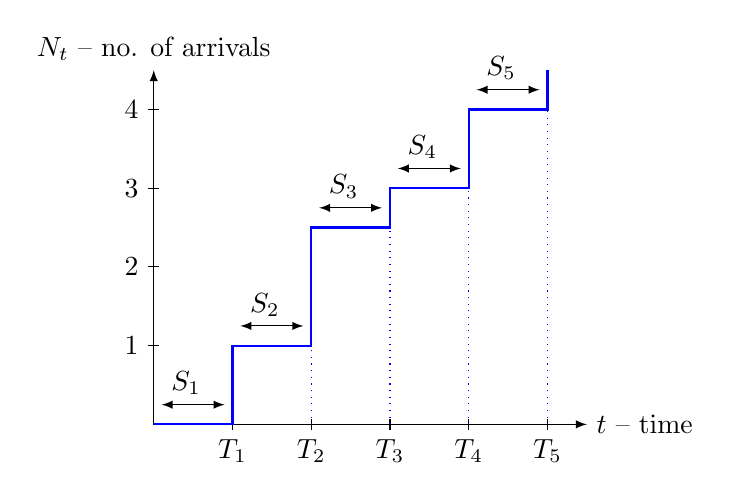
\begin{tikzpicture}[>=latex]
    \draw [<->] (0, 4.5) node [above] {$N_t$ -- no. of arrivals} |-
    (5.5, 0) node [right] {$t$ -- time};
    \foreach \x [evaluate=\x as \y using \x] in {1,...,5} \draw
    (\x,2pt) -- (\y, -2pt) node [below] {$T_{\x}$};
    \foreach \x [evaluate=\x as \y using \x] in {1,...,4} \draw
    (2pt,\x) -- (-2pt, \y) node [left] {\x};
    \draw [blue,thick] (0,0) -| (1,1) -| (2,2.5) -| (3,3) -| (4,4) -| (5,4.5);
    \draw [blue,dotted] (2,0) -- (2,1);
    \draw [blue,dotted] (3,0) -- (3,2.5);
    \draw [blue,dotted] (4,0) -- (4,3);
    \draw [blue,dotted] (5,0) -- (5,4);
    \draw [<->] (0.1,0.25) node [above right] {$S_1$} -- (0.9,0.25);
    \draw [<->] (1.1,1.25) node [above right] {$S_2$} -- (1.9,1.25);
    \draw [<->] (2.1,2.75) node [above right] {$S_3$} -- (2.9,2.75);
    \draw [<->] (3.1,3.25) node [above right] {$S_4$} -- (3.9,3.25);
    \draw [<->] (4.1,4.25) node [above right] {$S_5$} -- (4.9,4.25);
  \end{tikzpicture}
\end{center}

Each $T_i$ for $i = 1,2,3,4,5$ represents an arrival and generally,
each arrival time is defined as

\begin{displaymath}
  T_n = \sum_{i=1}^{n} S_i
\end{displaymath}

where the interarrival times
$S_1,S_2,\ldots,S_n \overset{\textrm{iid}}{\sim} Exponential(\lambda)$.
Thus, every $S_i$ has the probability density function

\begin{displaymath}
  f_{S_i}(t) = \lambda e^{\lambda t};\ t > 0;\ i=1,2,3,\ldots
\end{displaymath}

and cumulative distribution function

\begin{displaymath}
  F_{S_i}(t) = 1 - e^{-\lambda t}
  .
\end{displaymath}

\begin{definition}[Number of Arrivals]

  \begin{displaymath}
    N_t =
    \begin{cases}
      \max_{n \geq 1} \{n \mid T_n \leq t\} & t \geq 0 \\
      0 & t < T_1
    \end{cases}
  \end{displaymath}

\end{definition}

\begin{itemize}
  \item Recall: $Exponential(\lambda)$ is a memoryless RV
    \begin{enumerate}
      \item $F_{\tau}(t) =
        \begin{cases}
          1 - e^{-\lambda t} & t \geq 0 \\
          0 & t < 0
        \end{cases} \Rightarrow f_{\tau}(t) = \lambda e^{-\lambda t}$
      \item $\E\left[\tau\right] = \frac{1}{\lambda}$ and $\Var(\tau)
        = \frac{1}{\lambda^2}$
      \item $P(\tau > t + s \mid \tau > s) = P(\tau > t)$
      \item $P(\tau \leq t + \epsilon \mid \tau > t) = \lambda
        \epsilon +o(\epsilon);\ \lim_{\epsilon \rightarrow 0} \frac{o(\epsilon)}{\epsilon} = 0$
    \end{enumerate}
\end{itemize}

\begin{proof}

  \begin{align*}
    P(\tau > t + \epsilon \mid \tau > t) &= P(\tau > \epsilon) \\
                                         &= e^{-\lambda \epsilon} \\
                                         &= 1 - \lambda \epsilon + o(\epsilon)
  \end{align*}

\end{proof}


\chapter{Statistical Inference}

\section{Detection \& Bayes' Theorem}

Consider $N$ possible exclusive causes of a particular health symptom.

\begin{center}
  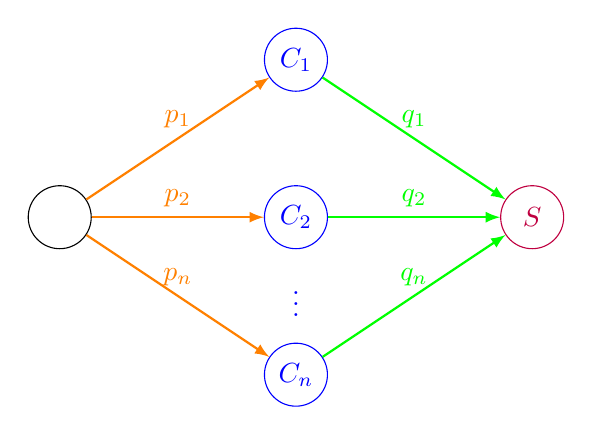
\begin{tikzpicture}[
      >=latex,
      node/.style={
        draw,circle,minimum size=0.8cm,inner sep=0pt
      },
    ]
    \node[node] (pr) at (0,0) {};
    \node[node,color=blue] (c1) at (3,2) {$C_1$};
    \node[node,color=blue] (c2) at (3,0) {$C_2$};
    \node[,color=blue] (dots) at (3,-1) {$\vdots$};
    \node[node,color=blue] (cn) at (3,-2) {$C_n$};
    \node[node,color=purple] (s) at (6,0) {$S$};
    \draw[thick,->,color=orange] (pr) -- (c1) node[anchor=south,midway] {$p_1$};
    \draw[thick,->,color=orange] (pr) -- (c2) node[anchor=south,midway] {$p_2$};
    \draw[thick,->,color=orange] (pr) -- (cn) node[anchor=south,midway] {$p_n$};
    \draw[thick,->,color=green] (c1) -- (s) node[anchor=south,midway] {$q_1$};
    \draw[thick,->,color=green] (c2) -- (s) node[anchor=south,midway] {$q_2$};
    \draw[thick,->,color=green] (cn) -- (s) node[anchor=south,midway] {$q_n$};
  \end{tikzpicture}
\end{center}

\begin{itemize}
  \item Each cause $i$ has a prior probability $p_i$ and it has a
    probability $q_i$ of causing the observed symptom.
  \item We want to esimate the \underline{posterior probability}
    $\pi_i$ of cause $i$ given the symptom $S$,
    \begin{equation*}
      \pi_i = \Prb\left(C_i \mid S\right) = \frac{\Prb\left(C_i \cap S\right)}{\Prb\left(S\right)} = \frac{\Prb\left(S \mid C_i\right)\ \Prb\left(C_i\right)}{\sum_{j} \Prb\left(S \mid C_j\right)\ P\left(C_j\right)}
    .\end{equation*}
    From the diagram above the posterior distribution for cause $i$
    can be simplified to
    \begin{equation}
      \pi_i = \frac{q_i\ p_i}{\sum_j q_j\ p_j}
    .\end{equation}
\end{itemize}

\section{MAP \& MLE}
\begin{definition}[Maximum a posteriori (MAP)]
  \begin{displaymath}
    \MAP \triangleq \argmax_i\ \pi_i = \argmax_i\ p_i\ q_i
  \end{displaymath}
\end{definition}
\begin{definition}[Maximum Likelihood Estimation (MLE)]
  \begin{displaymath}
    \MLE \triangleq \argmax_i q_i \equiv \MAP \text{ assuming uniform priors }\ p_i = \frac{1}{N}\ \forall i
  \end{displaymath}
\end{definition}
More generally, if $X,Y$ are discrete RVs then
\begin{align*}
  \MAP\left[X \mid Y=y\right] &= \argmax_x\ \Prb\left(X=x \mid Y=y\right) \\
  \MLE\left[X \mid Y=y\right] &= \argmax_x\ \Prb\left(Y=y \mid X=x\right)
\end{align*}
\begin{itemize}
  \item Called detection because everything is discrete, i.e.,
    detection and classification are synonymous.
  \item MAP: which cause best explaisn the observed symptom.
  \item MLE: which cause best generates/induces the observed symptom.
\end{itemize}
\begin{example}[MAP/MLE Analysis of BSC]
  Consider a $\BSC\left(p\right)$ with $p < \frac{1}{2}$.
\end{example}
\begin{center}
  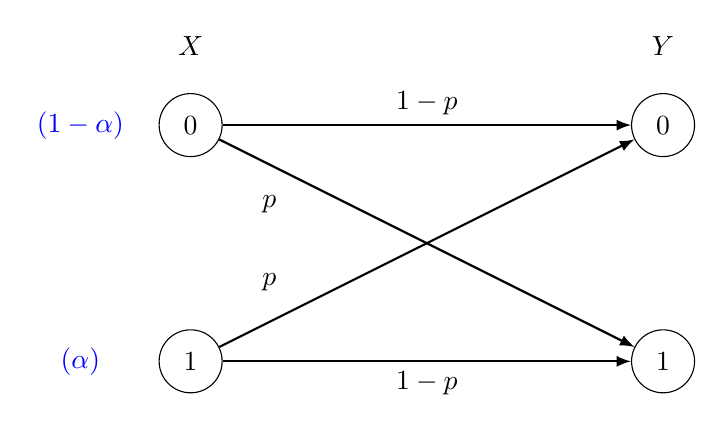
\begin{tikzpicture}[
      >=latex,
      node/.style={
        draw,circle,minimum size=0.8cm,inner sep=0pt
      },
    ]
    \node[node] (x0) at (0,0) {$0$};
    \node[node] (y0) at (6,0) {$0$};
    \node[node] (x1) at (0,-3) {$1$};
    \node[node] (y1) at (6,-3) {$1$};
    \node at (0,1) {$X$};
    \node at (6,1) {$Y$};
    \node[color=blue] at (-1.4,0) {$\left(1-\alpha\right)$};
    \node[color=blue] at (-1.4,-3) {$\left(\alpha\right)$};
    \node at (1,-1) {$p$};
    \node at (1,-2) {$p$};
    \draw[thick,->] (x0) -- (y0) node[anchor=south,midway] {$1-p$};
    \draw[thick,->] (x1) -- (y1) node[anchor=north,midway] {$1-p$};
    \draw[thick,->] (x0) -- (y1);
    \draw[thick,->] (x1) -- (y0);
  \end{tikzpicture}
\end{center}
\begin{center}
  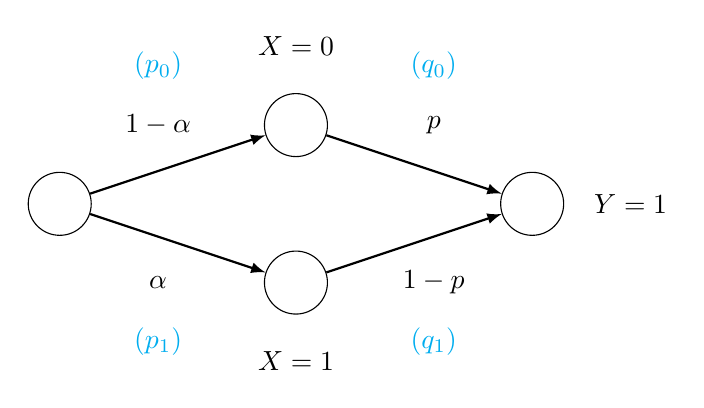
\begin{tikzpicture}[
      >=latex,
      node/.style={
        draw,circle,minimum size=0.8cm,inner sep=0pt
      },
    ]
    \node[node] (pr) at (0,0) {};
    \node[node] (x0) at (3,1) {};
    \node[node] (x1) at (3,-1) {};
    \node[node] (y1) at (6,0) {};
    \draw[thick,->] (pr) -- (x0);
    \draw[thick,->] (pr) -- (x1);
    \draw[thick,->] (x0) -- (y1);
    \draw[thick,->] (x1) -- (y1);
    \node[color=cyan] at (1.25,1.75) {$\left(p_0\right)$};
    \node[color=cyan] at (1.25,-1.75) {$\left(p_1\right)$};
    \node at (1.25,1) {$1-\alpha$};
    \node at (1.25,-1) {$\alpha$};
    \node[color=cyan] at (4.75,1.75) {$\left(q_0\right)$};
    \node[color=cyan] at (4.75,-1.75) {$\left(q_1\right)$};
    \node at (4.75,1) {$p$};
    \node at (4.75,-1) {$1-p$};
    \node at (3,2) {$X=0$};
    \node at (3,-2) {$X=1$};
    \node at (7.25,0) {$Y=1$};
  \end{tikzpicture}
\end{center}
\begin{equation*}
  \Rightarrow \MAP\left[X \mid Y=1\right] = \argmax_{i \in \{0,1\}}\ p_i q_i
.\end{equation*}
This yields the inequality statement,
\begin{equation*}
  p_0 q_0 \overset{\hat{X}_1=0}{\underset{\hat{X}_1=1}{\lessgtr}} p_1 q_1
\end{equation*}
where $\hat{X}_1$ is the $\MAP$ estimate of $X$ when $Y=1$ is $0$
or $1$. Thus
\begin{equation*}
  \left(1-\alpha\right) p\ \overset{0}{\underset{1}{\lessgtr}}\ \alpha \left(1-p\right)
\end{equation*}



\end{document}
